\documentclass[10pt]{article}
\usepackage[margin=1.8cm]{geometry}
\usepackage{amsmath}
\usepackage{booktabs}
\usepackage{graphicx}
\usepackage{caption}
\usepackage[hidelinks]{hyperref}
\setlength{\parskip}{0.3em}
\setlength{\parindent}{0pt}
\captionsetup{font=small}

\title{\vspace{-1.5em}Benchmarking Approximate Nearest Neighbour Search\\\large CS4.406 Assignment 3 (individual)}
\date{}

\begin{document}
\maketitle
\vspace{-2em}

\textbf{Machine.} Intel Core i7-13620H (10 cores, 16 threads), 16 GB RAM, Windows 11. Only the CPU was used. The RTX 4050 is not used because \texttt{faiss-cpu} has no GPU support. \textbf{Software.} Python 3.13.2, FAISS 1.15.1 (CPU), NumPy 2.2.3, h5py 3.16.0, Matplotlib 3.10.1. \textbf{Data.} ann-benchmarks SIFT-1M (Euclidean) and GloVe-100 (normalised, Euclidean). Operating points are chosen on queries 1--5000 and all numbers are measured on queries 5001--10000. Recall@10 counts ties at the 10th distance as hits, using exact distances recomputed from the raw vectors. Speed is queries per second (QPS), one query per call, one thread, median of three repeats.

\section{Part 1: exact baseline}
Exact FAISS search matches the stored neighbours (recall@10 = 1.000000 on both datasets). Unit tests cover the recall function (8 tests, all passing).

\begin{center}
\begin{tabular}{lrrr}
\toprule
Dataset & Single query, 1 thread (QPS) & Batch of 5000, 1 thread (QPS) & Batch of 5000, 16 threads (QPS) \\
\midrule
SIFT-1M & 10.2 & 128.4 & 167.5 \\
GloVe-100 & 9.7 & 111.8 & 160.1 \\
\bottomrule
\end{tabular}
\end{center}

A single query streams all $Nd$ floats from memory for about $2Nd$ floating-point operations, so it is limited by memory bandwidth and is slow. A batch becomes a matrix product $QX^\top$. That reuses each block of $X$ across many queries and runs at BLAS speed, giving about 11--13$\times$ more QPS on one thread. Adding threads helps only 1.3--1.4$\times$. I did not profile why; the top-$k$ selection after the product is one likely limit.

\section{Part 2: three indexes}
\begin{figure}[h]
\centering
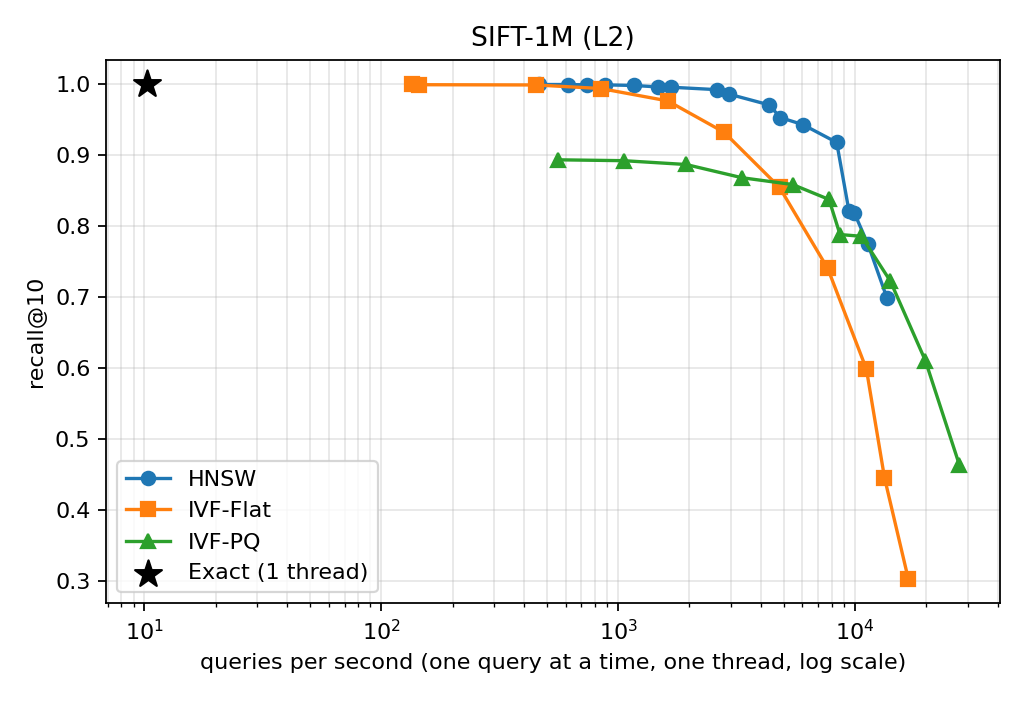
\includegraphics[width=0.46\linewidth]{../results/figures/recall_vs_qps_sift.png}
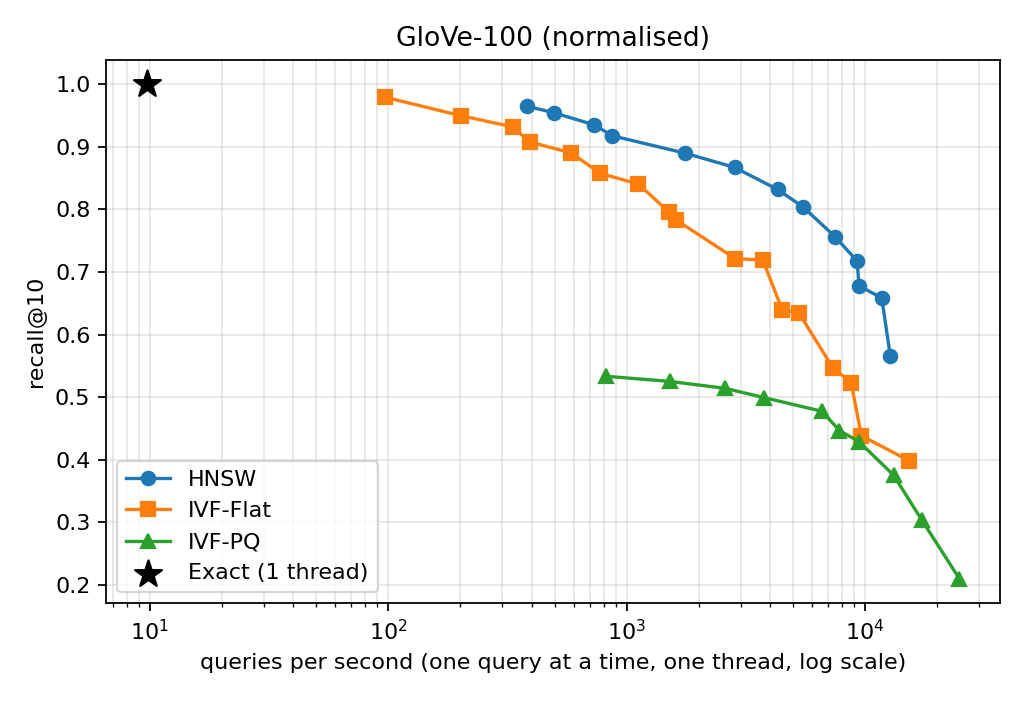
\includegraphics[width=0.46\linewidth]{../results/figures/recall_vs_qps_glove.png}
\caption{Recall@10 against QPS on the reporting half. Lines are the Pareto frontier over build settings (HNSW $M\in\{8,16,32\}$; IVF-Flat and IVF-PQ $\texttt{nlist}\in\{1024,4096\}$, PQ $m$). The star is exact search.}
\end{figure}

\begin{center}
\resizebox{0.85\linewidth}{!}{\begin{tabular}{llrr}
\toprule
Dataset & Index & QPS @ recall 0.90 & QPS @ recall 0.95 \\
\midrule
SIFT-1M (L2) & Exact & \multicolumn{2}{r}{10.2 (no recall loss)} \\
SIFT-1M (L2) & HNSW & 8373.1 & 4207.9 \\
SIFT-1M (L2) & IVF-Flat & 2802.9 & 1620.8 \\
SIFT-1M (L2) & IVF-PQ & not reached & not reached \\
GloVe-100 (normalised) & Exact & \multicolumn{2}{r}{9.7 (no recall loss)} \\
GloVe-100 (normalised) & HNSW & 731.1 & 496.1 \\
GloVe-100 (normalised) & IVF-Flat & 392.0 & 96.4 \\
GloVe-100 (normalised) & IVF-PQ & not reached & not reached \\
\bottomrule
\end{tabular}
}
\end{center}

\begin{center}
\resizebox{\linewidth}{!}{\begin{tabular}{llllrrr}
\toprule
Dataset & Index & Build setting & Param & Build (s) & Index (MiB) & Bytes/vector \\
\midrule
SIFT-1M (L2) & HNSW & M=32 & efSearch=48 & 104.9 & 747.8 & 784.1 \\
SIFT-1M (L2) & IVF-Flat & nlist=4096 & nprobe=64 & 75.8 & 497.9 & 522.1 \\
SIFT-1M (L2) & IVF-PQ & -- & -- & -- & -- & -- \\
GloVe-100 (normalised) & HNSW & M=32 & efSearch=384 & 359.6 & 758.6 & 672.2 \\
GloVe-100 (normalised) & IVF-Flat & nlist=1024 & nprobe=256 & 9.5 & 460.9 & 408.4 \\
GloVe-100 (normalised) & IVF-PQ & -- & -- & -- & -- & -- \\
\bottomrule
\end{tabular}
}
\end{center}
\textit{Index size and bytes per vector include stored raw vectors where the index keeps them (HNSW and IVF-Flat). Build time is wall-clock time for the whole build, not profiled. IVF-PQ rows are empty because no setting reached 0.95.}

\textbf{Why IVF-PQ cannot reach high recall.} IVF-PQ ranks candidates by $\sum_j T_j[\mathrm{code}_j]$, which is a sum of sub-space quantisation errors. Nearest-neighbour distances are small relative to that error, so the true top-10 is interleaved with vectors that look slightly closer. Recall stops rising once every probed cell has been scanned: SIFT reaches 0.59 at $m=16$ and 0.75 at $m=32$, and GloVe reaches 0.32 at $m=10$ and 0.53 at $m=20$. Adding $m$ halves the error per sub-space and helps, but without exact re-ranking the ceiling stays below 0.90 for these settings. The Part 3 compression experiment would address this; I did not run it.

\textbf{Build-setting note.} On SIFT, HNSW reaches 0.95 at $M=32$, efSearch = 48. On GloVe, it needs efSearch = 384 at $M=32$, and $M=8$ never reaches 0.85. The high-dimensional, less-clustered GloVe vectors need a denser graph.

\section{Part 3: scaling on SIFT (Scaling option)}
\begin{figure}[h]
\centering
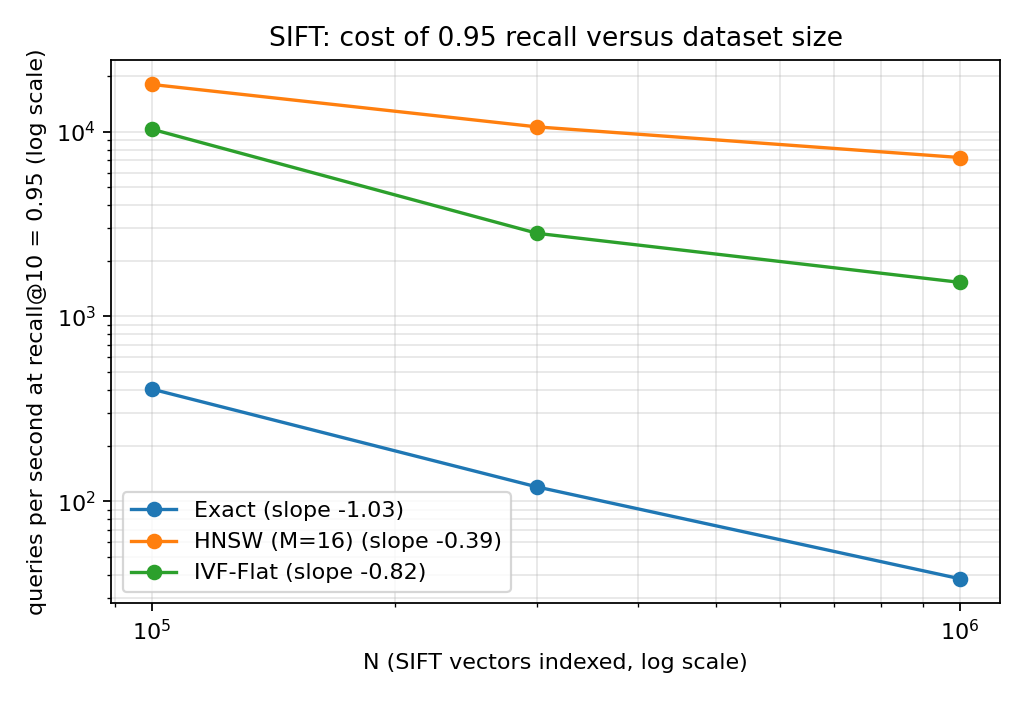
\includegraphics[width=0.42\linewidth]{../results/figures/scaling_sift.png}
\hspace{1em}
\begin{minipage}[c]{0.5\linewidth}
\resizebox{\linewidth}{!}{\begin{tabular}{lrrr}
\toprule
Index & $N$ & QPS @ recall 0.95 & Slope vs $N$ \\
\midrule
Exact & 100,000 & 404.4 & -1.03 \\
Exact & 300,000 & 119.3 & -1.03 \\
Exact & 1,000,000 & 38.1 & -1.03 \\
HNSW (M=16) & 100,000 & 18025.3 & -0.39 \\
HNSW (M=16) & 300,000 & 10618.0 & -0.39 \\
HNSW (M=16) & 1,000,000 & 7250.5 & -0.39 \\
IVF-Flat & 100,000 & 10320.3 & -0.82 \\
IVF-Flat & 300,000 & 2817.5 & -0.82 \\
IVF-Flat & 1,000,000 & 1530.2 & -0.82 \\
\bottomrule
\end{tabular}
}
\end{minipage}
\caption{Cost of recall@10 = 0.95 against $N$. Settings: HNSW $M=16$; IVF-Flat $\texttt{nlist}=\mathrm{round}(4\sqrt{N})$. Ground truth is recomputed for each $N$.}
\end{figure}

\textbf{Hypothesis test.} The exact-search slope is $-1.03$, as predicted. The HNSW slope is $-0.39$, at the edge of the predicted $[-0.4,-0.1]$. The IVF-Flat slope is $-0.82$, not the predicted $-0.5$. The refutation condition in \texttt{hypothesis.md} applies: the nprobe needed for recall 0.95 rose from 32 at 100K to 64 at 300K and 1M, because the grid is coarse and the required value sits between steps. Vectors scanned per query, $\texttt{nprobe}\cdot N/\texttt{nlist}$, grew about 6.3$\times$ over the 10$\times$ increase in $N$, which matches the measured slope. The mechanism is the probe count, not the list size.

\section{Part 4: dimension of uniform random vectors (own data)}
\begin{figure}[h]
\centering
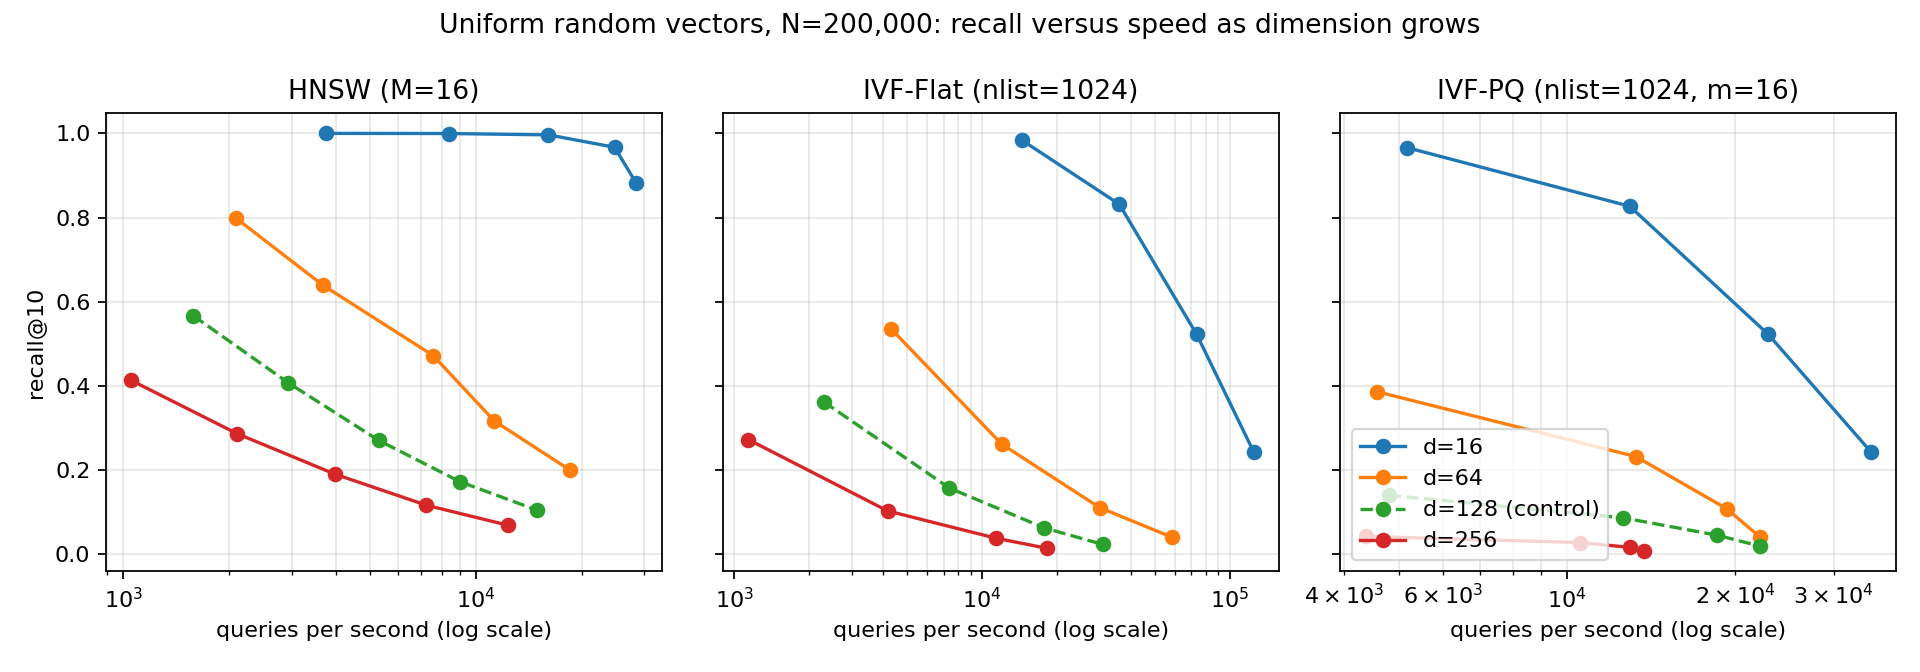
\includegraphics[width=0.95\linewidth]{../results/figures/part4_dimension.png}
\caption{Uniform vectors in $[0,1]^d$, $N=200$K, 1000 queries. Recall@10 against QPS for each dimension $d$ (dashed line: control $d=128$). Build settings are fixed; search grids are fixed.}
\end{figure}

\begin{center}
\resizebox{0.95\linewidth}{!}{\begin{tabular}{lrrrrr}
\toprule
$d$ & Relative contrast & HNSW recall (efSearch=64) & IVF-Flat recall (nprobe=16) & IVF-PQ recall (nprobe=16) & Exact NN distance / mean \\
\midrule
16 & 2.839 & 0.997 & 0.832 & 0.827 & 0.352 \\
64 & 1.481 & 0.472 & 0.261 & 0.232 & 0.675 \\
128 (control) & 1.292 & 0.270 & 0.157 & 0.086 & 0.774 \\
256 & 1.188 & 0.190 & 0.102 & 0.027 & 0.842 \\
\bottomrule
\end{tabular}
}
\end{center}

I changed only the dimension, using settings 16, 64, 256 and a control at 128. Relative contrast (mean distance over nearest-neighbour distance) falls from 2.84 to 1.19, as predicted, so the nearest neighbour is hard to separate from typical points. At a fixed budget, recall falls for all three indexes. The mechanism is loss of contrast, which makes small errors in the search path return non-neighbours. H1 and H2 held. H3 held in part: at $d=64$ HNSW (0.47) beats IVF-Flat (0.26) and IVF-PQ (0.23), but at $d=256$ HNSW is also weak (0.19), and the IVF indexes lose more recall in relative terms. Not tested: other $N$, clustered or non-uniform data, and PQ settings beyond $m=16$.

\section{Part 5: report answers}
\textbf{1. Fastest at recall 0.95.} HNSW on both datasets: 4208 QPS on SIFT and 496 QPS on GloVe, against 1621 and 96 for IVF-Flat. IVF-PQ never reached 0.95. The answer does not change, but the margin does: HNSW leads IVF-Flat by 2.6$\times$ on SIFT and 5.1$\times$ on GloVe. IVF-Flat needs 256 of 1024 lists probed on GloVe, against 64 of 4096 on SIFT. My explanation is that GloVe's clusters are less separated, so partitioning finds fewer of the true neighbours, though I did not measure cluster quality directly.

\textbf{2. Build and memory.} HNSW builds took 60--105 s on SIFT and 360--715 s on GloVe, using about 650--790 bytes per vector. IVF-Flat builds took 9--76 s at about 410--520 bytes per vector. IVF-PQ at $m=16$ uses about 26 bytes per vector and at $m=32$ about 42 bytes, against 512 for raw float32 SIFT, roughly a 12--20$\times$ saving. PQ gives up the recall ceiling described above.

\textbf{3. What Parts 3 and 4 show.} Headline numbers mislead when they are measured at one dataset size or on one distribution. Scaling showed IVF-Flat's advantage over HNSW grows with $N$. The dimension experiment showed the same index at the same settings goes from 0.997 to 0.19 recall as contrast drops. A benchmark on SIFT alone would overstate what an ANN index achieves on harder data, and the single-query, single-thread protocol hides the batch speedup that exact search gets.

\textbf{4. Choice for 150K and 10M vectors, 100 ms per query, 16 GB.} At 150K, exact single-thread search at 100K ran at 404 QPS, so about 3.7 ms per query at 150K. That is well inside 100 ms with recall 1.0, so I would use exact search and no index. At 10M, exact search is about 26 ms per query at 1M and would scale to about 260 ms single-threaded, over budget. I would use HNSW with $M=32$, tuned to recall at or above 0.95 on held-out queries. At 1M, HNSW reached 0.95 at about 7250 QPS, or about 0.14 ms per query. Under the slope of $-0.39$ measured in Part 3, that would be about 0.3 ms at 10M. Raw float32 vectors take about 5 GB at 10M $\times$ 128 dimensions, and the $M=32$ graph adds roughly 2.4 GB (about 236 bytes per vector, from the 1M build), so it fits in 16 GB. The 10M estimates are extrapolations and I did not run that size.

\textbf{5. Two ways the benchmark could mislead.} (a) The recall function trusted distances the index returned. For IVF-PQ these are approximate, which inflated recall. I found this during Part 4, when IVF-PQ showed 0.999 recall at $d=128$ while IVF-Flat showed 0.16 with the same probes. Recall is now recomputed from exact distances. The earlier IVF-PQ numbers are still in the git history. I tested this with the unit tests and by checking the corrected values. (b) The speed numbers come from one thread and one query per call, and include Python call overhead. A deployed system may batch queries and use more threads, which could change the ranking. I did not test batched or multi-threaded ANN timing. I also used a single query split and a single random seed for Part 4, so the variance of the measurements is unknown.

\end{document}
